\label{chap:system_overview}
This chapter provides the reader with an overview of IRLED electronics. Firstly, it discusses the Close Support Electronics (CSE) hardware used to drive IRSP systems in order to give the reader an understanding of the internal flow of data from within a CSE externally to an array. Then, it discusses the communication within an overall IRLED system at a block level to provide the reader with a high level understanding of the flow of communication from input (scene generation) to output (array) in different system configurations.

\section{Close Support Electronics}
    \label{sec:close_support_electronics}
    As mentioned briefly in Chapter~\ref{chap:background}, a CSE is needed to drive IRLED arrays. Conceptually, A CSE is an interface that converts digital display data to an array specific format in order to produce IR imagery. From there it converts formated data from the digital domain to analog and amplifies analog signaling to drive an array by charging the internal array cells that make up an array. It further provides power for an array, and regulates the current in order to safe guard arrays from physical damage due to misconfiguration or heating.

    The TCSA, NSLEDS, and HDILED arrays discussed in Chapter~\ref{chap:background} can all be driven using the same electronics with the only difference in the boards directly attached to the hybrid array. Figure~\ref{fig:sleds_block} shows the internal components of the CSE broken out in green. In typical configurations, a display system drives a CSE using dual HDMI inputs to increase the system bandwidth and achieve higher frame rates. Typically, these will each carry half of a frame segmented either vertically or horizontally. Each input decodes the video signals in parallel and then outputs individual pixels that are then routed into the main FPGA board which houses a Xilinx Vertex 6 FPGA\cite{XILINX1}. From there, pixels are routed into an internal buffered directly or decoded (in the case of PDP) and then buffered. Other interfaces may be utilized in place of HDMI as will be discussed later in this section.

    \begin{figure}
        \centering
        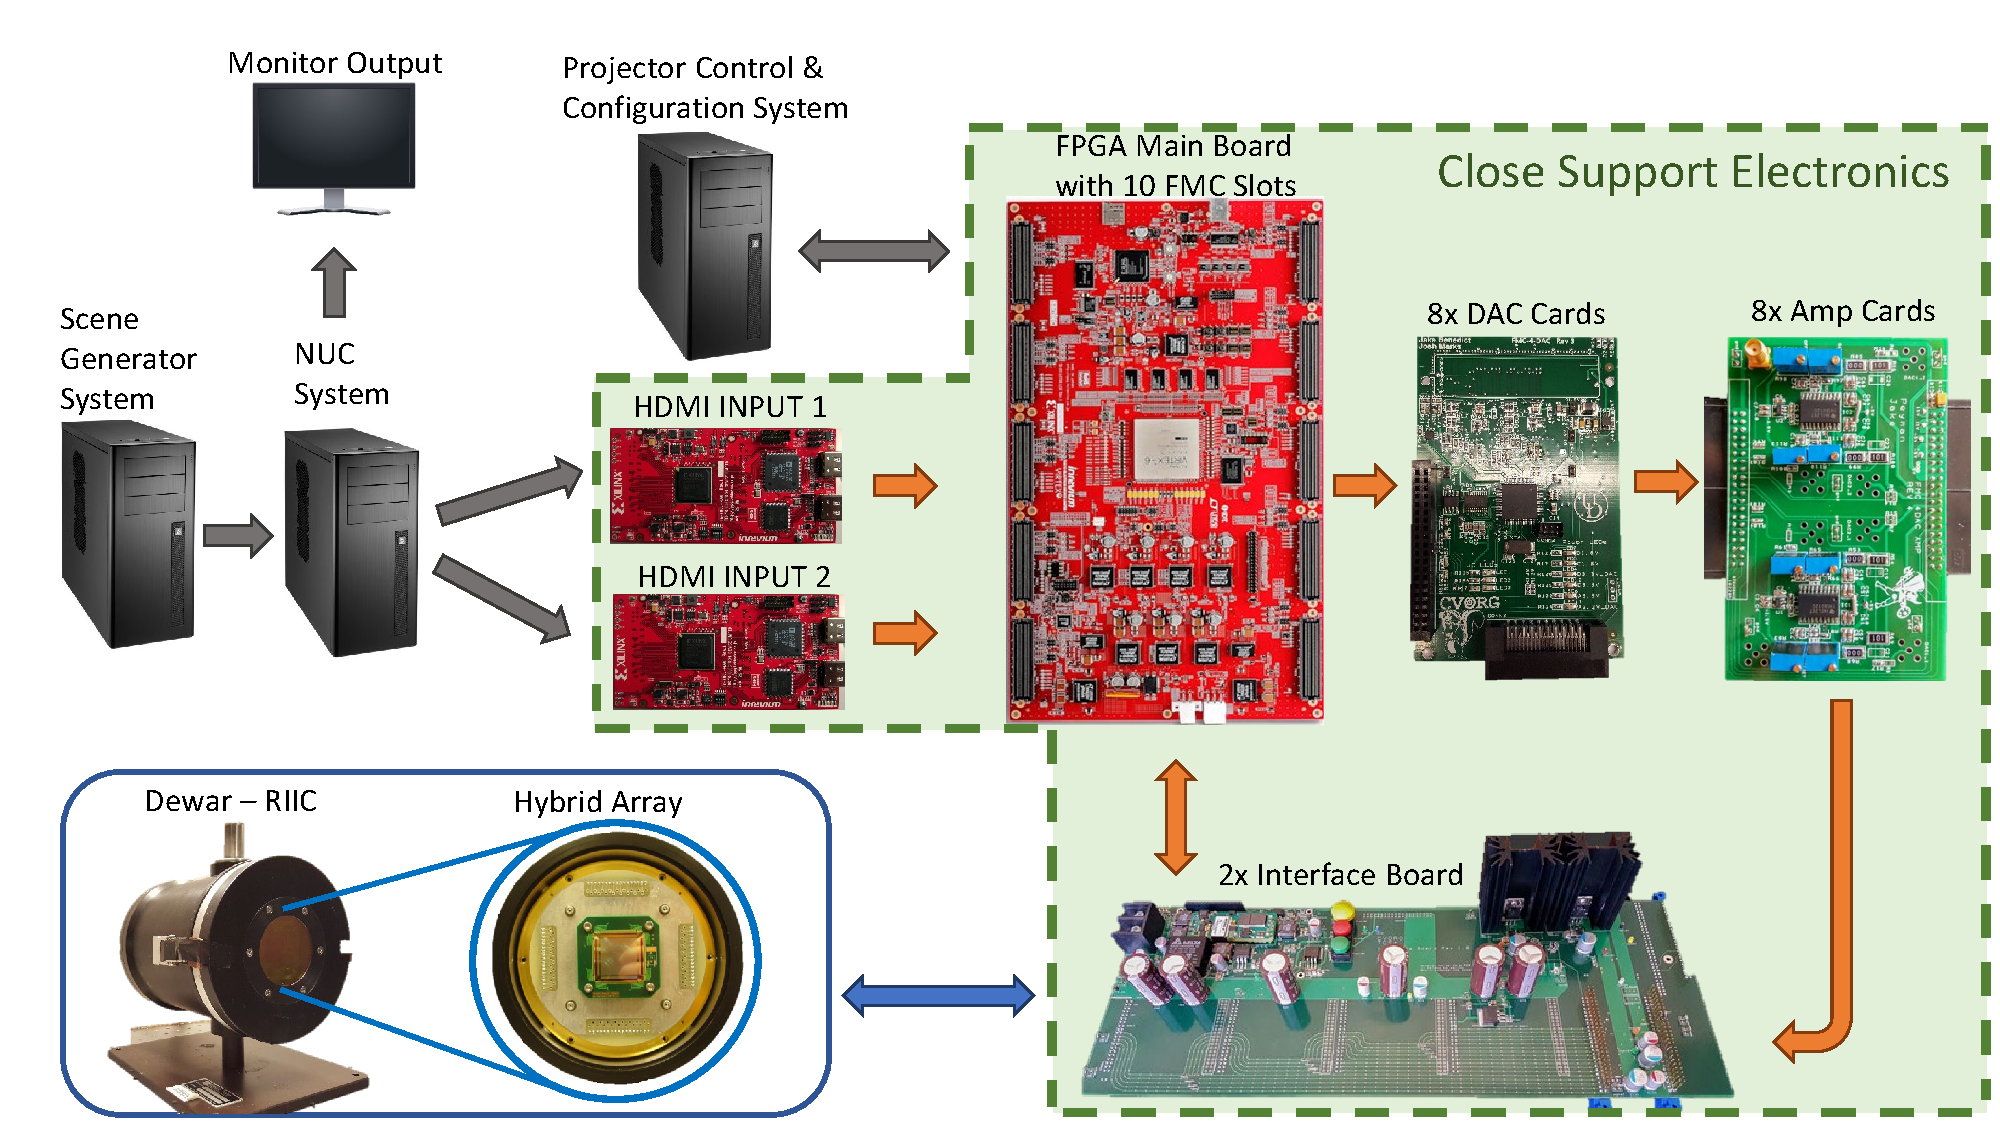
\includegraphics[width=0.67\textwidth]{fig/sleds_block.pdf}
        \caption{SLEDS System Block Diagram}
        \label{fig:sleds_block}
    \end{figure}

    Due to the two input cards, the firmware within the main FPG board is responsible for multiplexing between both inputs to draw data to an array without allowing for the internal firmware buffers to overflow. In practice, current firmware does this by buffering the minimal amount of data needed for a write from both inputs in parallel and context switches between the inputs every other write or every two writes depending on the configuration. As long as the buffers are sized large enough to accommodate for the time needed for the array write process to finish for an individual write, then overflow should not occur. Additional logic is provided to query and detect internal buffer overflows in cases of misconfiguration or signal integrity faults. In practice, if an overflow fault occurs, it is visually obvious in recorded IR data as well.

    Once enough data is buffered for one of the inputs, the firmware will control the write process to drive the 8 DAC cards which each house 2 16-bit DAC integrated circuits per card, with each circuit consisting of 2 channels per DAC. Yielding 32 parallel channels with 512 total signals. Once the DAC process is done, the analog output of the 32 channels is then routed to 8 amplifier card which contain 4 amplifiers each. Following this, the amplified signals are routed through 2 interface boards which contain ribbon cables that attach to an array hybrid. The ribbon cabling carries both the amplified signals as well as other control signals from the firmware that are routed directly from the main FPGA board to one of the interface boards.

    Figure~\ref{fig:nessie_enclosure_internals} shows the components installed within a CSE chassis. Multicolored ribbon cables are shown in the top right. Mounted to the bottom is the main FPGA board. The two large boards at the top are the 2 interface boards with 8 amplifier cards plugged into them along the bottom. The boards in between the FPGA are and amplifer cards are the DAC boards. The power supply is on the left.

    The additional control signals provided by the firmware and routed to the RIIC through these cables are discussed in Chapter~\ref{sec:array_Interleaved_write_process}. The specifics of the PDP firmware architectures write process are discussed in Chapter~\ref{chap:implementation}.

    \begin{figure}
        \centering
        \includegraphics[width=1.0\textwidth]{fig/nessie_enclosure_internals.jpg}
        \caption{CSE Internals}
        \label{fig:nessie_enclosure_internals}
    \end{figure}

\section{Communication Flow}
    In this section, a discussion of internal CSE communication will be provided followed by a discussion of external communication within an IRLED projector system as a whole.

    \subsection{Internal CSE Communication}
        Figure~\ref{fig:cse_comm_block} shows the internals of CSE communication. Communication for controlling the behavior of CSE is done through a daisy chained set of UART devices utilizing a reliable blocking two way communication protocol called the CVORG protocol\footnote{Named after my research group at the University of Delaware.}. Without loss of generality, the protocol itself consist of commands to control various aspects of operation, such as, tripping an array, setting voltage limits, and configuring firmware operation. It also allows for information to be retrieved about current system configuration, as well as, operational errors. The destination of an operation is encoded as part of each command. Thus, commands not meant for a given component are forwarded along the chain. When commands are issued by a system, they are encoded for transport via the CVORG protocol and sent over UART. The system will then wait for an acknowledgment potentially containing payload data. When a command has finished executing within a CSE, it will send the acknowledgment over UART to the command initiator with requested payload data or simply as a receipt indicating that an action has been successfully executed. The underlying implementation details of the CVORG protocol itself are beyond the scope of this work and will not be discussed here.

        Memory mapped I/O between the frontend and backend firmware is controlled by the microblaze soft processor and used to control the underlying PDP firmware registers, as well as, program an array using Serial Peripheral Interface (SPI) (Not shown). The details of command operations will be discussed in Chapter~\ref{sec:frontend_arch}. Additionally, SPI communication is also used to send data for LCD readout. Typically this includes voltage and current information, as well as, the results of power on sanity checks. Finally, the details of the processing performed on HDMI display data sent directly to the Backend Firmware within PDP will be discussed in Chapter~\ref{sec:backend_arch}. Earlier non-PDP firmware implementations utilized within the TCSA, NSLEDS, and HDILED arrays also utilized HDMI but contained a different less robust implementation. These are outside of the scope of this thesis and will not be discussed here.

        \begin{figure}
            \centering
            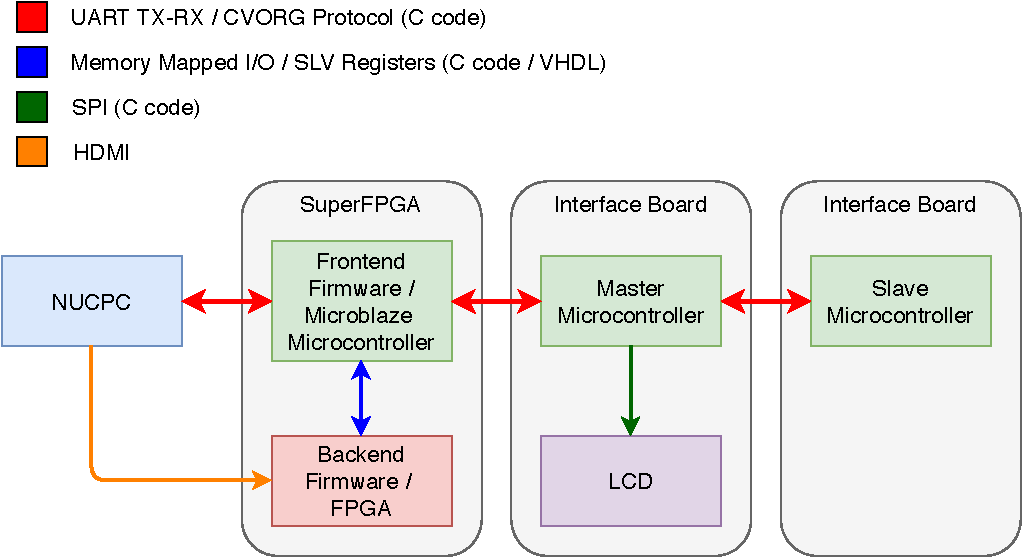
\includegraphics[width=1.0\textwidth]{fig/cse_comm_block.pdf}
            \caption{CSE Internal Communication Block Diagram}
            \label{fig:cse_comm_block}
        \end{figure}

    \subsection{External System Communication}
        Figures~\ref{fig:external_cse_comm_direct}, \ref{fig:external_cse_comm_half_indirect}, and \ref{fig:external_cse_comm_indirect} show the details of external communication to a CSE in various different system configurations. These provide a representation of some general types of setups that an IRLED array may be placed in. In general, a scene generator of some form would be utilized in all cases to provide IR scene imagery for an array to display. In all the configurations, a Low Pin Count (LPC) FPGA Mezzanine Card (FMC) connector provides the ability for various interfaces to be used to send data to the CSE, such as serial protocols or display based protocols over different types of hardware links. The FMC interface cards are responsible for retrieving the data over the link and formatting it in a manner that the internal CSE FPGA can decode.

        In practice, in display protocol setups, 24-bit pixel words and a data enable pin are utilized, but there is no hardware limitation and other word sizes could be used in setups that utilized other types of interfaces. A vertical sync signal can also be utilized to reset pixels every display frame in display protocol setups. As mentioned earlier in this section, current CSE setups utilize two HDMI FMC cards for input where the input for the top half of an array will be delivered over one cable and the bottom over the other.

        For example, in the NSLEDS array, input would be split into two 512 by 1024 display streams operating in parallel. API communication on the other hand utilizes UART and the CVORG protocol and is largely the same process for all arrays. Generally speaking, on start, frontend software would configure the firmware to output for the correct array size and program the array. After which, auxiliary functionality such as tripping and untripping the array would typically be the only strictly necessary communication done over UART.

        High-speed serial interfaces are currently in development in order to provide more control over the timing of data sent to CSEs within systems. These would allow for the blanking data inherit in display based protocols to be removed altogether\footnote{Blanking is discussed in Chapter~\ref{chap:display_protocols}.}, as well as, provide users with a means to send data only when required as opposed to at a strictly static interval controlled by vendor drivers such as is the case with GPUs.

        Figure~\ref{fig:external_cse_comm_direct} depicts direct communication in which formated scene data is sent directly to a CSE and system configuration is done directly by a scene generator. In this type of setup, the scene generator can monitor CSE operation directly, as well as, operate in either a closed or open loop type setup\cite{nagrath2009control,frank2018control}.

        \begin{figure}
            \centering
            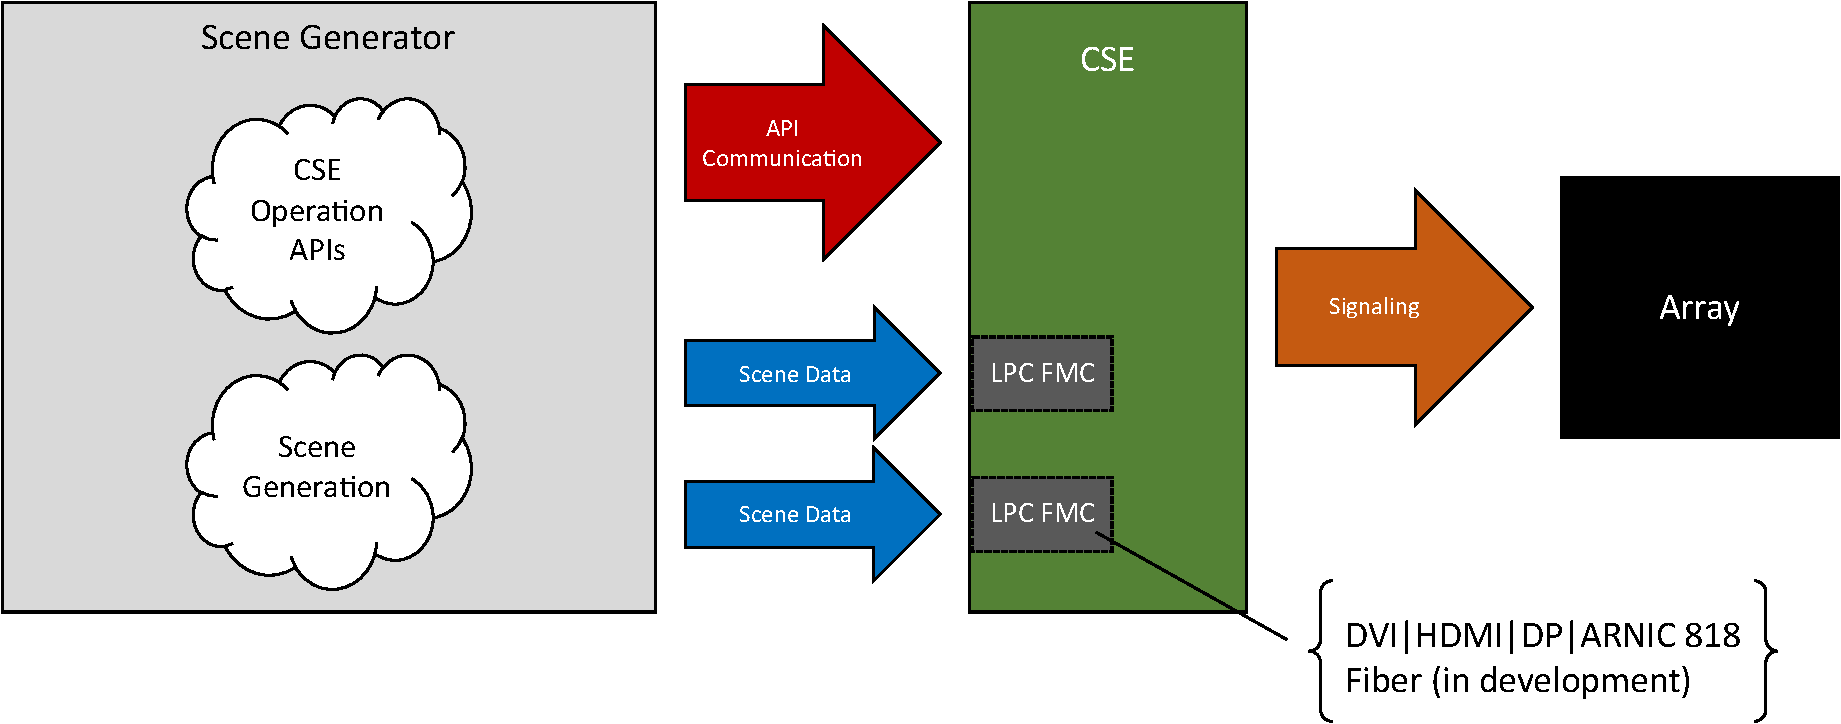
\includegraphics[width=1.0\textwidth]{fig/external_cse_comm_direct.pdf}
            \caption{CSE External Direct Communication Block Diagram}
            \label{fig:external_cse_comm_direct}
        \end{figure}

        A direct communication setup is desirable for minimizing end-to-end latency within an system for use cases where performance is paramount. For example, closed loop scenerios may feed recorded output imagery from an array back into the scene generator for in the loop analysis or in some cases subsequent frames may depend on the recorded results from prior frames. This means that in many cases subframe latency is desireable in that individual components in a system should not require buffering entire frames anywhere in the system as this would introduce a latency of a frame or more from generation to capture. This would necessarily result in the system needing delayed feedback control\cite{hu2002dynamics}. This represents a complex problem to solve in practice. It becomes even more difficult if the frame delays are unpredictable and dynamic from frame to frame forcing the scene generators to compensate in some manner, such as, sending off frames\footnote{An off frame is simply an empty frame that can be analyzed to check if frames are arriving at the expected time or if a frame slip or unexpected delay has occurred.} between imagery to characterize delay and detect unexpected behavior, as well as, provide a means of resynchronization between a scene generator and camera or sensor.

        Figure~\ref{fig:external_cse_comm_half_indirect} depicts indirect API communication in which system configuration is done through client APIs, and scene data is sent directly to a CSE. This type of setup is useful for situations where control over a CSE is needed but where API operation cannot be tightly coupled with a scene generator due to development costs or practical reasons. Similar to the direct setup, end-to-end latency is minimized by directly driving an array.

        \begin{figure}
            \centering
            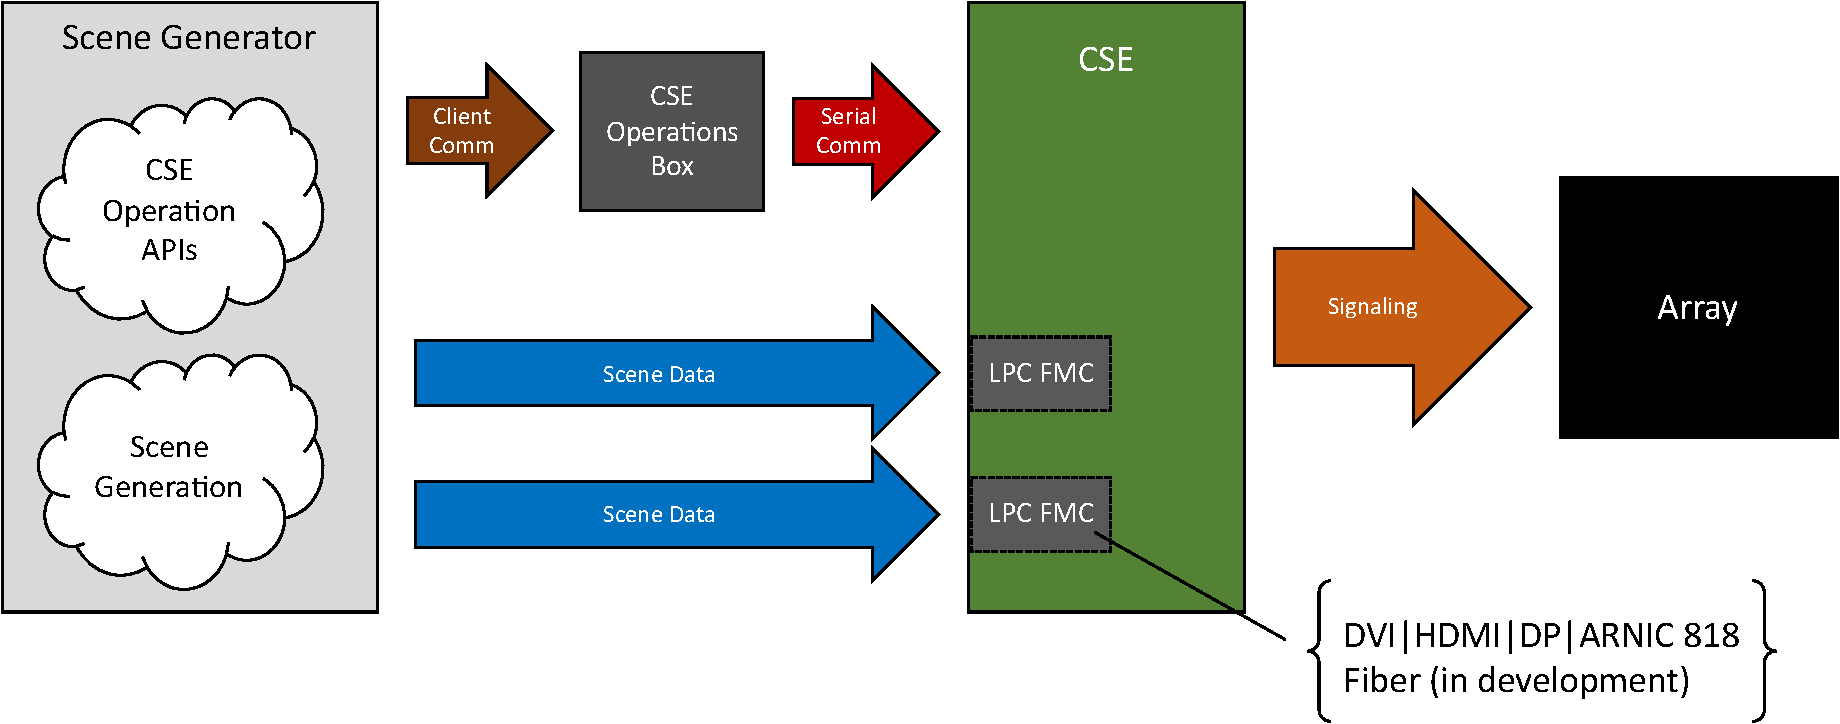
\includegraphics[width=1.0\textwidth]{fig/external_cse_comm_half_indirect.pdf}
            \caption{CSE External Indirect API Communication Block Diagram}
            \label{fig:external_cse_comm_half_indirect}
        \end{figure}

        In an indirect API communication setup, thin client API shims are provided to execute commands using remote procedure calls (RPC) which then are executed within a CSE operations box to communicate with the CSE. This API shims provide the same interface and level of control as the direct API communication but are simply issued through some indirect layer such as ethernet or infinaband. When a shim command is issued it encoded and transmitted to the CSE Operation Box. The CSE operation xox then maps the shim command into a direct command call (as if it were being executed directly by a scene generator) and sends it to a CSE. Then the CSE operation box waits for a response from the CSE. Once a response has arrived from the CSE it will encode it and transmit it back to the scene generator, which is analogous to the direct operation of the CVORG with a middleman in between.

        Figure~\ref{fig:external_cse_comm_indirect} depicts an indirect setup in which both API communication and scene data are sent to an intermediate CSE operations box. Similarly, to the indirect API communication setup, client API shims are provided to execute commands using remote procedure calls (RPC) which then are executed within a CSE operations box to communicate with the CSE.

        \begin{figure}
            \centering
            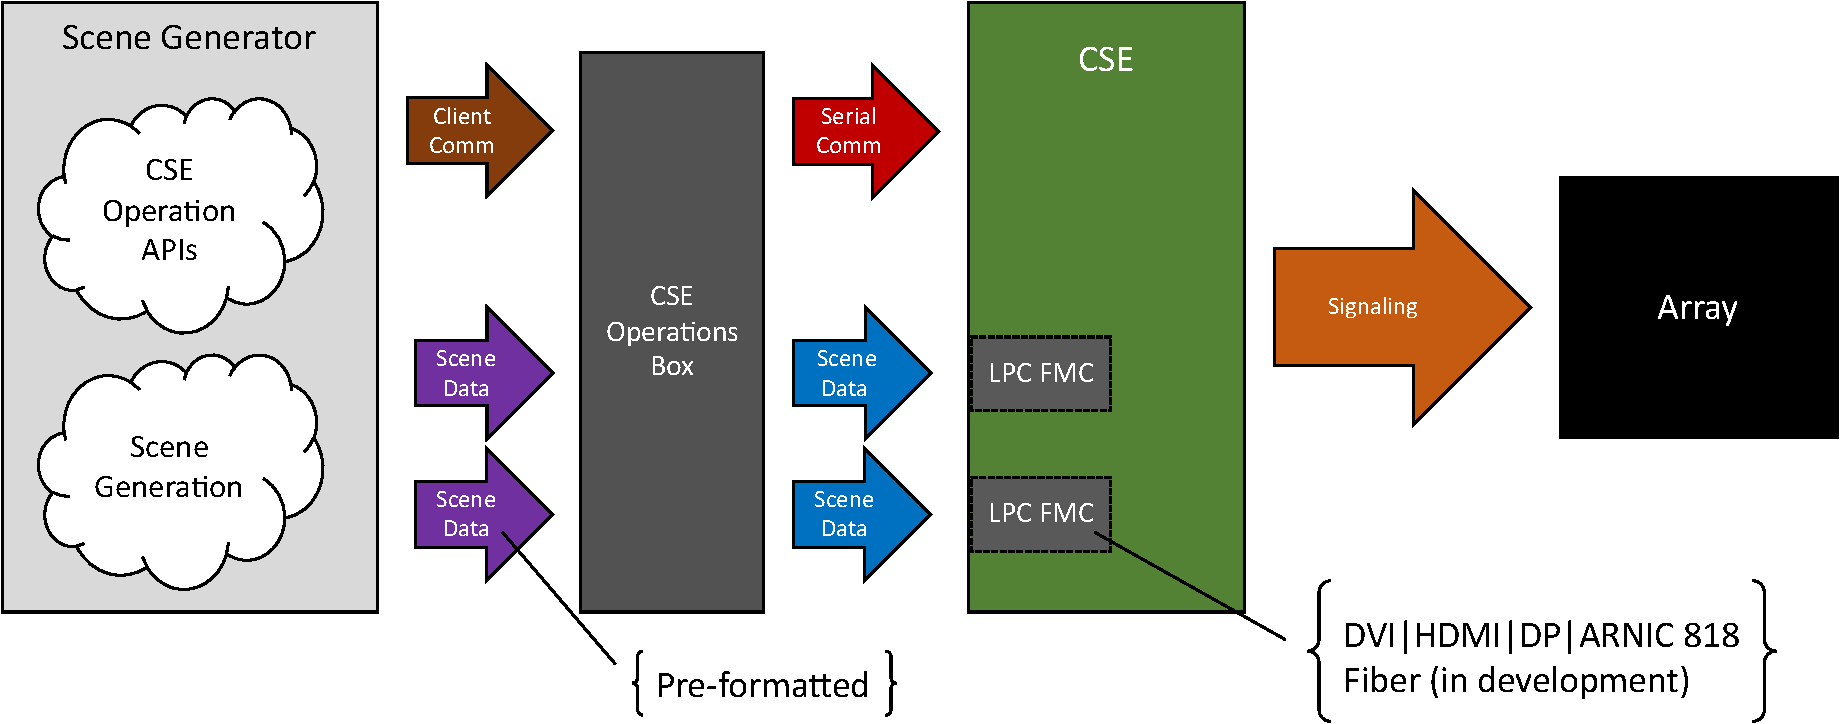
\includegraphics[width=1.0\textwidth]{fig/external_cse_comm_indirect.pdf}
            \caption{CSE External Indirect API and Data Communication Block Diagram}
            \label{fig:external_cse_comm_indirect}
        \end{figure}

        An indirect data and API communication setup is utilized in the event that data cannot be formatted directly for display on an array within a scene generator. It may also be utilized in cases where non-uniformity correction is performed externally from scene generation as shown in Figure~\ref{fig:sleds_block}. However, this would result in an additional latency cost that could complicate synchronization in closed loop setups due to delayed feedback control being required. A third scenerio where this type of setup may be used is without a scene generator, where a CSE operation box could be used as a test bed to characterize an array directly, as well as, to test and troubleshoot operations. Imagery itself also could be displayed directly from the CSE operation box. This may be desireable in some open loop setups where the recording and processing of data is performed separately as this means no additional infrastructure would be required to be developed by users to interface with a CSE. Instead, users could utilize the provided infrastructure with little to no development costs.

        In closing, there are many different possible system setups in which IRLED projector systems can be utilized depending on user application and requirements. A well design IRLED system will ease the process of incorporating a new projector within an environment through versatility while minimizing performance impact, as well as, providing users with an clear picture of the tradeoffs associated with each type of setup.

        While this chapter covered the flow of communication inside and outside a CSE, as well as, different system setups in order to provide the reader with an understanding of the challenges and complexities of utilizing and driving IRLED arrays, Chapter~\ref{chap:array_write_process} shifts focus to discuss the hardware details of IRLED arrays' write process and the formatting of data sent to arrays to provide context on some of the challenges of writing to an IRLED array.
